%\documentclass[pre,amsmath,amssymb, twocolumn, showpacs]{revtex4-1}
\documentclass{iopart}
%showpacs, twocolumn
\usepackage{dcolumn}
\usepackage{bm}
\usepackage{graphicx}
\usepackage{hyperref}
\usepackage{mathptmx}
\usepackage{subfigure}
\usepackage[utf8]{inputenc}
\usepackage{bbold}
\usepackage{color}
\newcommand{\david}[1]{{\color{red} #1}}
\newcommand{\ata}[1]{{\color{blue} #1}}
\newcommand{\pp}{p_{al}}
\makeatletter

\newcommand{\eqref}[1]{(\ref{#1})}

\begin{document}

\title{Efficient algorithms for the periodic Lorentz gas in two and three dimensions}

\author{Atahualpa S.~Kraemer$^{1}$, Nikolay Kryukov$^{2}$ and David P.~Sanders$^{2}$}

\address{$^{1}$ Institut für Theoretische Physik II - Soft Matter
Heinrich-Heine-Universität Düsseldorf
Building 25.32
Room O2.56
Universitätsstrasse 1
D-40225 Düsseldorf, Germany\\
$^{2}$Departamento de F\'isica, Facultad de Ciencias, Universidad Nacional
Aut\'onoma de M\'exico,
Ciudad Universitaria, M\'exico D.F.\ 04510, Mexico
}

\eads{\mailto{ata.kraemer@gmail.com}, \mailto{kryukov@ciencias.unam.mx}
and 
  \mailto{dpsanders@ciencias.unam.mx}} \date{\today}


\begin{abstract}

We present efficient algorithms to calculate collisions for a periodic Lorentz gas in two and three dimensions. The 2D algorithm uses continued fractions to obtain the exact disc with which a particle will collide at each step, instead of using periodic boundary conditions. The 3D version uses the 2D algorithm by projecting to coordinate planes. We study the efficiency of the algorithms, and, as an application, calculate distributions of free paths for three different geometries.
\end{abstract}

\maketitle

\section{Introduction}



Lorentz gases are simple physical systems that present deterministic chaos \cite{cvitanovic1992investigation}, and are a popular model in statistical mechanics and nonlinear dynamics. This model consists of point particles that move freely until they encounter obstacles, often spheres, where they undergo elastic collisions. 
%When these obstacles are arranged periodically at the vertices of a grid (``periodic Lorentz gas''), the model is equivalent to a Sinai billiard \cite{bunimovich1981statistical}.

These systems can have different configurations of obstacles, e.g., random arrangements \cite{latz1997lyapunov,dellago1997lyapunov, van1998chaotic} or quasiperiodic structure \cite{kraemer2013embedding,wennberg2012free}. However, due to its simplicity, the periodic case has been most widely studied; see, e.g., \cite{bunimovich1981statistical,bleher1992statistical, chernov1994statistical, gilbert2011diffusive}. In this case, the model is equivalent to a Sinai billiard  \cite{bunimovich1981statistical}. Many of the results obtained theoretically for these gases are in the limit where obstacles are very small, i.e., the so-called Boltzmann--Grad limit \cite{caglioti2003distribution, golse2012recent,boca2007distribution,golse2006periodic,caglioti2008boltzmann,caglioti2010boltzmann, golse2000distribution,marklof2008kinetic, bourgain1998distribution}. There are still many interesting open questions in this area
\cite{gilbert2009persistence,marklof2011periodic,nandori2014tail, dettmann2012new}.

The standard simulation method for periodic Lorentz gases is to reduce to a single cell with periodic boundary conditions, and, in the simplest case, an obstacle in the centre of the cell\cite{sanders2005fine, sanders2008normal}. However, this requires that the program check in each cell whether the particle collides with the obstacle in the cell, or if it will move to the next cell. 
%That implies solving at least two linear equations and one quadratic, then checking if the solution of the quadratic equation is real and finally taking the maximum value of the two or three results. 
If the obstacle is large, it is quite likely that the particle will collide each time it crosses into a new cell. However, for very small obstacles, this method becomes inefficient.

Instead, we would like to just find the coordinates of the next obstacle with which the particle will collide, given its initial position and velocity.
%As we will see in section \ref{algorithm} this is indeed the first solution of the Diophantine inequality:
%
%\begin{equation}
%|\alpha q+b-p|\leq  \frac{v^2}{v_x} r
%\end{equation}
%
%where $r$ is the radius of the obstacles, $q$ and $p$ are integer variables, and $\alpha$ and $b$ are two real numbers related to the position $\vec{x}$ and velocity $\vec{v}$ of the particle. 
This turns out to be  closely related to the best rational approximant to an irrational number, and  can be solved using the continued-fraction algorithm. 
 Continued fractions have often been used to provide information about the free path distribution of the periodic Lorentz gas in the Boltzmann--Grad limit \cite{caglioti2003distribution, golse2012recent,boca2007distribution,golse2006periodic,caglioti2008boltzmann, caglioti2010boltzmann, golse2000distribution, bleher1992statistical,chernov1994statistical}.
  An algorithm along these lines was previously developed: see comments in \cite{zacherl1986power}; however, it was never published %\footnote{T.~Geisel, private communication}.
[T.~Geisel, private communication].
 Caglioti and Golse developed a method to encode the trajectories of particles using the continued fraction algorithm and the so-called 3-length theorem \cite{caglioti2003distribution, golse2012recent}. 


However, Golse's algorithm works only if the particle leaves the surface of a disk. This restriction prevents the algorithm from being used in other geometries, such as quasiperiodic arrays, two incommensurate overlapping arrays of square lattices, or with different shapes of obstacles; such systems may produce a number of surprising effects \cite{marklof2014power}.  On the other hand, due to the construction of the algorithm, it is not possible to use it in higher dimensions, which, to quote Golse, is ``a notoriously more difficult problem''.

In this paper, we develop a general, efficient algorithm to find a collision with a 2D square lattice of discs starting from an arbitrary initial condition. We then use that 2D algorithm to develop an algorithm for a 3D simple cubic lattice by projecting to coordinate planes.

\section{Continued fractions}
\label{algorithm}

In this section, we derive the basis of the 2D algorithm using continued fractions.
Its goal is to calculate efficiently where the first collision of a particle will occur in a square lattice. Without loss of generality, we will use the lattice formed by the integer coordinates in the 2D plane. We wish to calculate the minimal time $t^{\ast}>0$, such that a collision occurs with some disc with centre $\vec{c}=(q,p)$, with $q$ and $p$ integers. The condition for a collision is then 
\begin{equation}
\|\vec{x_0}+\vec{v_0} \, t^{\ast} -  \vec{c} \| = r,
\label{eq:classical}
\end{equation}
where $r$ is the radius of the obstacle, and $\vec{x_0}$ and $\vec{v_0}$ are the initial position and velocity of the particle. The collision then occurs at the point 
$\vec{x_0}+\vec{v_0} \, t^{\ast}$.

\subsection{Collision with a disc}
The classical algorithm finds the intersection between a line, corresponding to the trajectory of 
the particle, and a circle, corresponding to the circumference of the disc, by solving the quadratic equation~\eqref{eq:classical} for $t^{\ast}$. A first improvement follows from observing that we may instead look for the intersection with another line, as follows. We denote by $(v_{1}, v_{2})$ the components of the particle's velocity. Without loss of generality, in the following we take the speed $\sqrt{v_{1}^{2} + v_{2}^{2}}$ to be 1 and $v_1>0$ and $v_2>0$; we can always rotate or reflect the system such that these conditions are satisfied, due to its symmetry (see below).

We write the equation of the particle's trajectory as $y=\alpha x+b$ and look for its intersection with the vertical line $x=q$. As shown in figure~\ref{fig:circle}, if $|\alpha q+b-p| = |b| < \delta := r/v_1$, then a collision will take place. Due to the periodic boundary conditions, we can always take $0 < b < 1$, so we need only solve $b<\delta$. 
%This gives us a tool to calculate with which obstacle the particle will collide. 

At each step, we do not need to apply periodic boundary conditions at every step; rather, we only need to check 
\begin{equation}
|\{ \alpha  q_n \}+b -1|< \delta, 
\label{eq:master}
\end{equation}
where $\{ \cdot \}$ denotes the fractional part, and $q_n=q_{n-1}+1$, where $q_1$ is the $x$-coordinate of the closest obstacle to the particle at $t=0$. Then, the first $q_n$ that satisfies this inequality will be $q$. To calculate $p$, we use that either $p=\lfloor \alpha q +b\rfloor$ or $p=\lfloor \alpha q +b\rfloor+1$

\begin{figure}
\centering
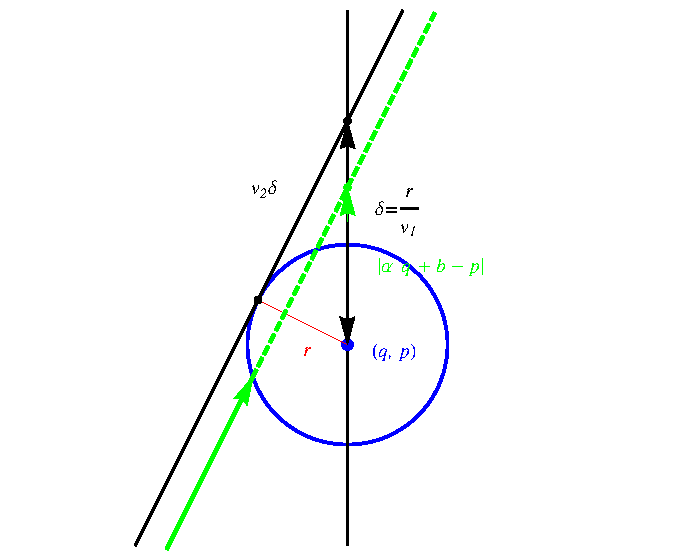
\includegraphics [width=240pt]{fig01.pdf}
\caption{Relation between the intersection of a line and a circle with integer coordinates and the intersection of the line $x = q$. }
\label{fig:circle}
\end{figure}


Now, to simplify the algorithm further, consider the integer coordinates $(q_n, p_n)$ such that
\begin{equation}
|\alpha q_n -p_n + b|< \delta,
\label{eq:1}
\end{equation}
and for any pair of numbers $(i,j)$ such that $i<q_n$, then $|\alpha i -j+ b|> \delta$,  $q=q_n$, and $p=p_n$. 
 
But $|\alpha q_i - p_i + b|$ are the distances between the integer coordinates $(q_i, p_i)$ and the point $( q_i ,\alpha q_i + b)$. Thus, we would like a sequence such that  
\begin{equation}
|\alpha q_i - p_i + b|<|\alpha q_{i-1} - p_{i-1} + b|
\label{eq:iteration}
\end{equation}
for every integer $i>1$. Also, the first pair of integer coordinates $q_0$ and $p_0$ should be $(0, 0)$ or $(0, 1)$, minimizing $| \alpha q_0 - p_0 + b |$, that is

\begin{eqnarray}
%|\alpha q_1 -p_1 + b|< f(b) = \begin{cases} b &\mbox{if } b < 1/2 \\ 
%1-b & \mbox{if } b > 1/2 \end{cases} .
|\alpha q_1 -p_1 + b|< f(b) =& b,  \quad \mbox{if } b < 1/2 \\ 
& 1-b,  \quad \mbox{if } b > 1/2.
\label{eq:prima}
\end{eqnarray}

Note that if $b < 1/2$, we have
$p_n= \lfloor \alpha q_n +b  \rfloor= \lfloor \alpha q_n  \rfloor $, if $b+\alpha q_n-\lfloor \alpha q_n  \rfloor < 1$, and  
$p_{n} = \lfloor \alpha q_n  \rfloor+1$, if  $b+\alpha q_n-\lfloor \alpha q_n  \rfloor > 1$.
Whereas if $b>1/2$, we  have $p_n= \lfloor \alpha q_n +b  \rfloor+1= \lfloor \alpha q_n  \rfloor+1$, if $b+\alpha q_n-\lfloor \alpha q_n  \rfloor < 1$ and 
$ p_{n} = \lfloor \alpha q_n  \rfloor+2$, if $b+\alpha q_n-\lfloor \alpha q_n  \rfloor > 1$. Substituting these four cases  in the two cases of equation \eqref{eq:prima}, we obtain that indeed $p_1= \lfloor \alpha q_1  \rfloor+1$. Iterating the inequality \eqref{eq:iteration} we obtain 
 %
\begin{equation}
 p_n= \lfloor \alpha q_n  \rfloor+1.
\label{eq:hn}
\end{equation}
 %
Combining the inequality \eqref{eq:1} with equation \eqref{eq:hn}, we obtain again equation \eqref{eq:master}. 

Thus, we have reduced the solution from two linear equations and one quadratic to one linear equation. Furthermore, now we do not check in every periodic cell, because if $\alpha >1$, for every $q_n$ we advance $\alpha$ cells. And we do not need to apply periodic boundary conditions until we reach the obstacle. 

\subsection{The Diophantine inequality: $|\alpha p - q|\leq \epsilon$}

Now, a better algorithm should find a way to find the set of $q_i$, such that inequality \eqref{eq:iteration} holds for every $i$, and there is no integer $q$  such that $q_i<q<q_{i-1}$ for some $i$ and
$|\{ \alpha  q_i \}+b -1|<|\{ \alpha  q \}+b -1| <|\{ \alpha  q_{i-1} \}+b -1|$. 

In order to do this, we can use the continued fraction algorithm to obtain solutions to the inequality $|\alpha q - p|\leq \epsilon$. This algorithm already gives a sequence of $(q_n,p_n)$ such that $|\alpha q_i - p_i|<|\alpha q_{i-1} - p_{i-1}|$ if $q_{i-1} <q_i$. So, if we turn our inequality \eqref{eq:prima} into this other inequality, we will find our algorithm just by using the continued fraction algorithm.
Indeed, using equation \ref{eq:hn} and the inequality \ref{eq:prima}, we obtain $|\{ \alpha  q_1 \} -1|< 2b$ if $b < 1/2$ or $<  2(1-b)$  if $b > 1/2$, 

which is almost the continued fraction inequality, except that $p_1$ is always equal to $\lfloor \alpha q_1  \rfloor+1$. 

%\begin{equation}
%|\alpha  q_1-p_1|< \begin{cases} 2b &\mbox{if } b < 1/2 \\  2(1-b) & \mbox{if } b > 1/2 \end{cases}
%\label{eq:master2}
%\end{equation}

\begin{eqnarray}
|\alpha  q-p|<  & 2b, \quad \mbox{if } b < 1/2 \\ 
& 2(1-b), \quad  \mbox{if }  b > 1/2 %\end{cases}
\label{eq:master2}
\end{eqnarray}


Now we can apply the continued fraction algorithm to obtain $p_1$ and $q_1$ of inequality \eqref{eq:master2}.  If ${\alpha q_1+b} < \delta$ or $1-{\alpha q_1+b} < \delta$, then we have found the center of the obstacle at $(p_1,q_1)$, with  $p_1=\lfloor \alpha q_1  \rfloor+1$; otherwise, we have not found it, but we know that if the center of collision is at $(p,q)$ then
$p\geq p_1$, and $q \geq q_1$. Hence, we can just use $(q_1,p_1)$ even if they do not satisfy inequality \ref{eq:iteration}. Redefining $b_i$ as $b_0=b$, $b_i=\{\alpha q_i+b\}$, we can calculate a succession of $(p_i,q_i)$. If $b_n<\delta$ the algorithm stops, and the collision will take place with the obstacle centred at the coordinates $(q_n,p_n)$.


\section{Complete 2D algorithm}

We now have the necessary tools to implement the algorithm. The source code may be found in the supplementary information.

We call \texttt{obstacle($\alpha$, b)} the function that gives the centre of an obstacle with which a particle collides that has initial position $(0,b)$ and positive velocity with slope 
$0 < \alpha <1$. This function uses the algorithm mentioned above. However, in general the particle's velocity does not satisfy these conditions, and will need to be converted into this form.

Suppose first that we do have the good conditions on the velocity. Then we use the classical algorithm for one step, or at most two steps. In the classical algorithm, collisions with an obstacle inside a periodic cell (a unit square) are calculated. If there is no collision, then the particle moves to the next wall of the cell and periodic boundary conditions are applied. Due to  the fact that the slope satisfies $0 < \alpha < 1$, after a maximum of 2 steps, the classical algorithm will return the position of a collision or a coordinate of the form $(n,b)$, that may be rewritten as $(0,b)$ when periodic boundaries conditions are applied. So, if we use first the classical algorithm, and then the function \texttt{obstacle($\alpha$, b)}, we obtain the coordinates of the obstacle of the next collision.  


Now we need only to transform the velocity into the correct form. To do so, we use the symmetry of the system, applying rotations and reflections and then, after obtaining the coordinates of the collision, use the inverse transformations to return to the original system. 
We need a transformation $\mathsf{R}$ that converts the velocity into a positive velocity with slope $0<\alpha<1$. Then, we redefine $v \rightarrow \mathsf{R} \cdot v$ and $x \rightarrow \mathsf{R} \cdot x$ and  apply the efficient algorithm described above to obtain the position of the obstacle $x_c$. Finally, we apply the inverse of $R$ to obtain the final values:  $v \rightarrow \mathsf{R}^{-1} \cdot v$, $x \rightarrow \mathsf{R}^{-1} \cdot x$ and $x_c \rightarrow \mathsf{R}^{-1} \cdot x_c$. Here, $\mathsf{R}$ is a transformation that depends on the velocity. 

If $|\alpha|>1$, we reflect using the reflection matrix
$\mathsf{M}_{\mathrm{refl}} := \left(\begin{array}{cc}
0 & 1\\
1 & 0
\end{array}\right)$.
If $v_x<0$ and $v_y>0$, or $v_x<0$ and $v_y<0$, or $v_x>0$ and $v_y<0$, we rotate the  through an angle $\pi/2$, $\pi$ or $3\pi/2$, respectively, using the rotation matrix 
$\mathsf{M}_\mathrm{rot}(\theta) := \left( \begin{array}{cc}
\cos \theta & \sin \theta\\
-\sin \theta & \cos \theta
\end{array} \right)$.
So, for example, if $v_y<v_x<0$, then $\mathsf{R} = 
\mathsf{M}_{\mathrm{refl}} \cdot M_{\mathrm{rot}}(\pi) = \left(\begin{array}{cc}
0 & -1\\
-1 & 0
\end{array}\right)$. 

Finally, to calculate the exact collision point, we use the classical method	 to obtain the intersection between a line and a circle, and from there the resulting post-collision velocity.

%The efficient algorithm, together with the classical algorithm for comparison, are implemented in the source code, REF ???
%
%\subsection{Explicit algorithm}
%
%Now we have all the necessary tools to implement the complete algorithm step by step. The Julia language \cite{julialang} is used; the source code is available at ???
%
%The function \texttt{frac($\alpha, \epsilon$)} calculates the first integers $(q,p)$ such that 
%$|\alpha q-p|<\epsilon$ by using the continued fraction algorithm; see the appendix. This is used to calculate which disc is hit by the following function
%
%Now, define the function \texttt{eff(m, b, r)} as follows: 
%\begin{verbatim}
%function eff(m, b, r)
%	kn = 0
%    b1 = b
%    epsilon = r*sqrt(m*m+1) 
%    if(b < epsilon || 1 - b < epsilon)
%        if b < BigFloat("0.5")
%			(q, p) = frac(m, 2.*b)
%		else
%			(q, p) = frac(m, 2.*(1. - b))
%		end
%		b = mod(m*q + b, 1)
%		kn += q
%    end  
%	while b > epsilon && 1 - b > epsilon
%		if b < BigFloat("0.5")
%			(q, p) = frac(m, 2.*b)
%		else
%			(q, p) = frac(m, 2.*(1. - b))
%		end
%		b = mod(m*q + b, 1)
%		kn += q
%	end
%	q = kn
%    p = int(m*q+b1)
%    return [q, p]
%end
%\end{verbatim}
%
%This function applies the continued fraction algorithm along with the inequality \ref{eq:master2} until the distance in the y-direction between the line and the integer coordinates $(q, p)$ is less than $\epsilon$. 
%
%Then, the algorithm to localize the first obstacle, with which a particle with velocity $\vec{v}$ and position $\vec{x}$ will collide, is as follows (in pseudocode): 
%
%\begin{verbatim}
%if (v is in quadrant I) then     
%   (q,p)=efficient_algorithm(m, b, delta)
%   p=int(m*q)+1
%else if (v is in quadrant II) then
%   m=-m                               
%   % reflect the system with 
%   %respect to y-axis 
%   (q,p)=efficient_algorithm(m, b, delta)
%   p=int(m*q)+1
%   m=-m                                
%   % reflect the system with 
%   %respect to y-axis
%   q=-q                                
%   % reflect the system with 
%   %respect to y-axis
%else if (v is in quadrant III) then
%   b=1-b                              
%   % reflect the system with 
%   %respect to the origin
%   (q,p)=efficient_algorithm(m, b, delta)
%   b=1-b                              
%   % reflect the system with 
%   %respect to the origin
%   p=-(int(m*q)+1)                               
%   % reflect the system with 
%   %respect to the origin
%   q=-q                               
%   % reflect the system with 
%   %respect to the origin
%else if (v is in quadrant IV) then
%   b=1-b                              
%   % reflect the system with 
%   %respect to the x-axis
%   m=-m                               
%   % reflect the system with 
%   %respect to the x-axis
%   (q,p)=efficient_algorithm(m, b, delta)             
%   b=1-b                              
%   % reflect the system with 
%   %respect to the x-axis
%   m=-m                               
%   % reflect the system with 
%   %respect to the x-axis
%   p=-(int(m*q)+1)                               
%   % reflect the system with 
%   %respect to the x-axis
%endif
%\end{verbatim}
%
%Using the technique mentioned above, which, for the initial position $(0, b), 0 < b < 1$ and for any initial velocity returns the integer coordinates of the obstacle of the first collision, we make the function \texttt{Lorentz(x, v, r)} that calculates the first collision of the particle in the 2D plane. In order to calculate the exact collision point and the velocity after the collision, we need to use the classical collision functions \texttt{collision} and \texttt{velo\_col}.
%

\section{3D algorithm}

We now turn to an efficient algorithm for calculating the next collision with a sphere in 3D on a simple cubic lattice. The algorithm works by projecting to 2D planes and using the 2D algorithm in each plane, as follows.

Suppose we project a particle trajectory in a 3D lattice onto one of the $x$--$y$, $x$--$z$ or 
$y$--$z$ planes. We will obtain a periodic square lattice with a 2D trajectory, but with a speed in that plane that is, in general, not $1$. 
Thus, we can apply the 2D algorithm for each of the 3 projections, and obtain the coordinates of 3 obstacles in the 3 projected planes where the first collision occurs.  

We now check whether the obstacle coordinates in these projections correspond to the \emph{same} 3D obstacle. If not, then we move the particle to the cell containing the obstacle that is furthest away (i.e., has the maximum collision time), and continue.

If the obstacle coordinates coincide correctly, i.e. the integer obstacle coordinates returned by the 2D algorithm for each plane coincide pairwise, then our 3D algorithm predicts that there is a collision. However, this may not be the case, due to the geometry, as follows.

Using the 2D continued fraction algorithm in one of the planes $xy$, $xz$ and $yz$ is equivalent to calculating the first collision with a cylinder orthogonal 
to that plane. Joining those coordinates together is equivalent to calculating a collision with the intersection of three orthogonal cylinders with the same radius. 
Figure~\ref{fig:collision} shows such an intersection of three cylinders (called a tricylinder or Steinmetz solid \cite{tricylinder1974}), together with a sphere of the same radius. The sphere is contained strictly inside the intersection of the cylinders. 
 
\begin{figure}
\centering
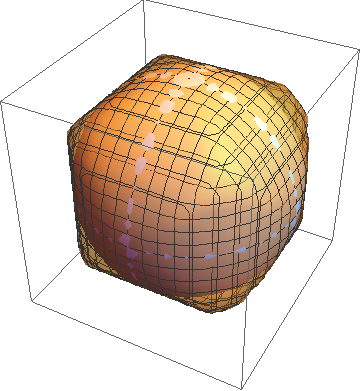
\includegraphics [width=240pt]{./region.png}
\caption{A sphere of radius $r$ embedded into the intersection of three orthogonal cylinders of the same radius. The volume inside the intersection but outside the sphere is the region where the 3D algorithm predicts false collisions.}
\label{fig:collision}
\end{figure}
 


Thus the algorithm may predict a false collision with the tricylinder, even though the particle does not actually collide with the sphere. To control this, we check if the particle really does collide with this obstacle by using the standard method; if so, then we have found a true collision; if not, we move the particle to the next cell and continue applying the algorithm. 
Numerically, we find the probability of a false collision to be around $0.17$. 
% Analytically, the sphere embedded in the tricylinder has the volume $V_{sph} = \frac{4}{3} \pi r^3$, while the tricylinder has the volume $V_{tc} = (16 - 8 \sqrt{2}) r^3$ \cite{tricylinder1974}. The probability of a false collision is therefore
% 
%$$ p_{false} = \frac{V_{tc} - V_{sph}}{V_{tc}} = 1 - \frac{\pi}{6 (2 - \sqrt{2})} \approx 0.106 $$

\section{Numerical measurements}

In order to test the efficiency of our algorithm, we measured the average time of the execution of the function finding the first collision starting from the initial point around the origin,
 depending on the radius of the obstacle, for both the classical and efficient algorithms.

\begin{figure}
\centering
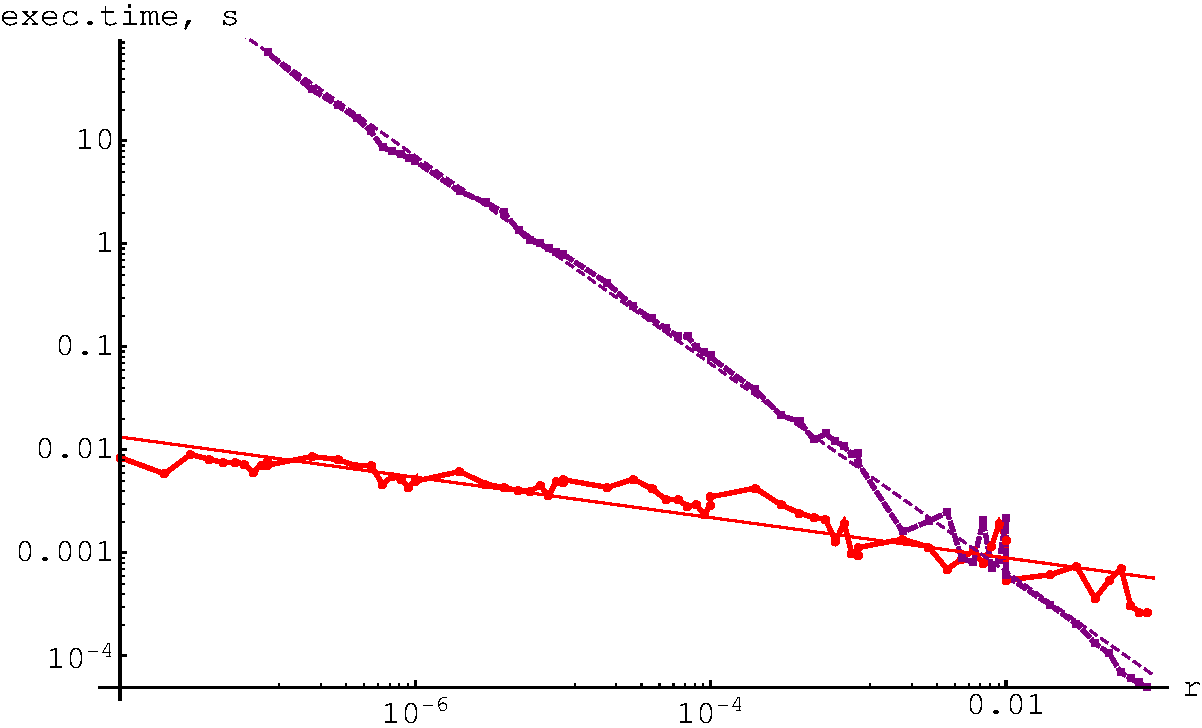
\includegraphics [width=260pt]{fig03.pdf}
\caption{Mean execution time to find the first collision in 2D Lorentz gas, for the classical (dotted curve) and efficient (solid curve) algorithms. The straight lines show power-law fits. }
\label{fig:time_2D}
\end{figure}

\begin{figure}
\centering
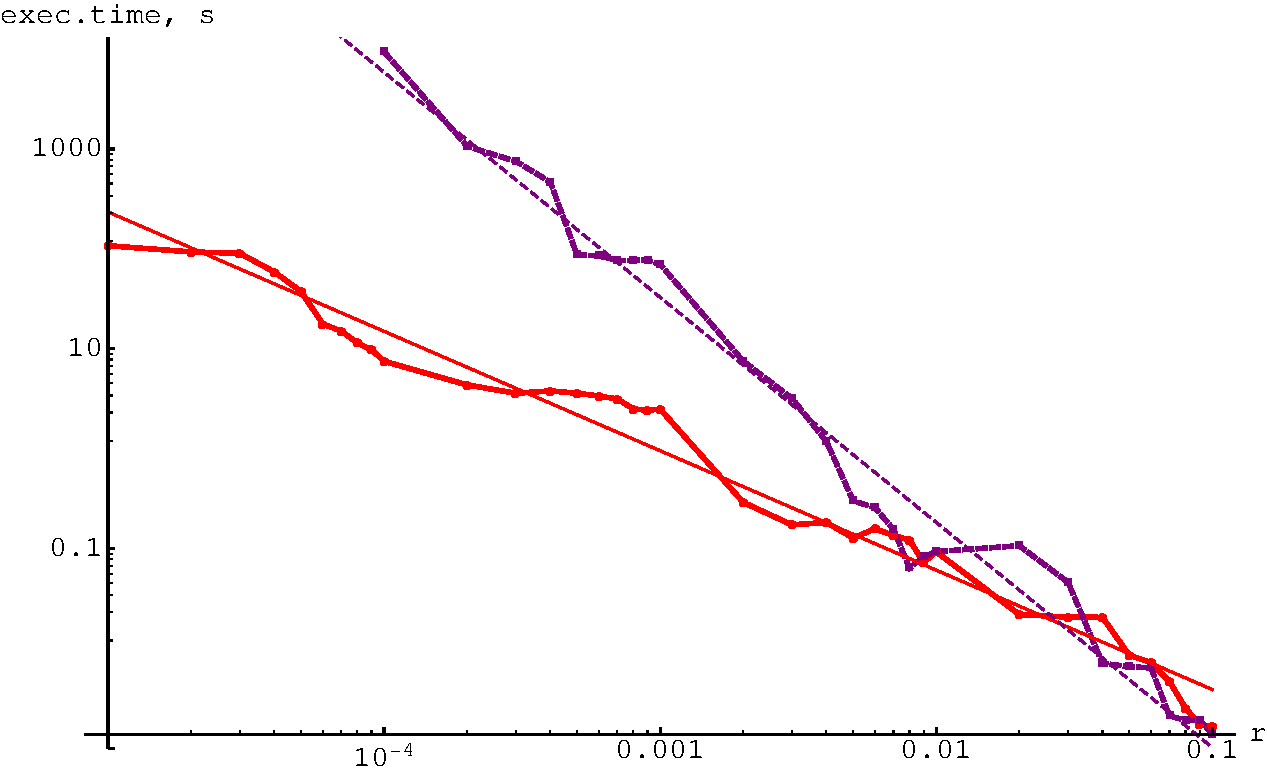
\includegraphics [width=260pt]{fig04.pdf}
\caption{Mean execution time to find the first collision in 3D Lorentz gas, for the classical (dotted curve) and efficient (solid curve) algorithms. The straight lines show power-law fits.}
\label{fig:time_3D}
\end{figure}

Figures \ref{fig:time_2D} and \ref{fig:time_3D} show the results for the 2D and 3D algorithms. We performed power-law fits for the execution time as a function of obstacle radius. For the 2D case, we found an exponent of $-1.01$ for the classical algorithm and $-0.20$ for the efficient algorithm. For the 3D case, the results were $-2.25$ and $-1.20$ for classical and efficient, respectively. As we can see, our algorithms are significantly more efficient for $r < 0.01$. 

Similarly, we calculated the execution time per cell as a function of the obstacle radius, for both the 2D and 3D efficient algorithms, with comparison to the corresponding classical algorithms; see Figures~\ref{fig:exectimepercell2D} and \ref{fig:exectimepercell3D}. Since the classical algorithms use periodic boundary conditions, the time per cell is basically constant, independent of the obstacle radius. 
For small radii, we again observe the efficiency of the new algorithms.

\begin{figure}
\centering
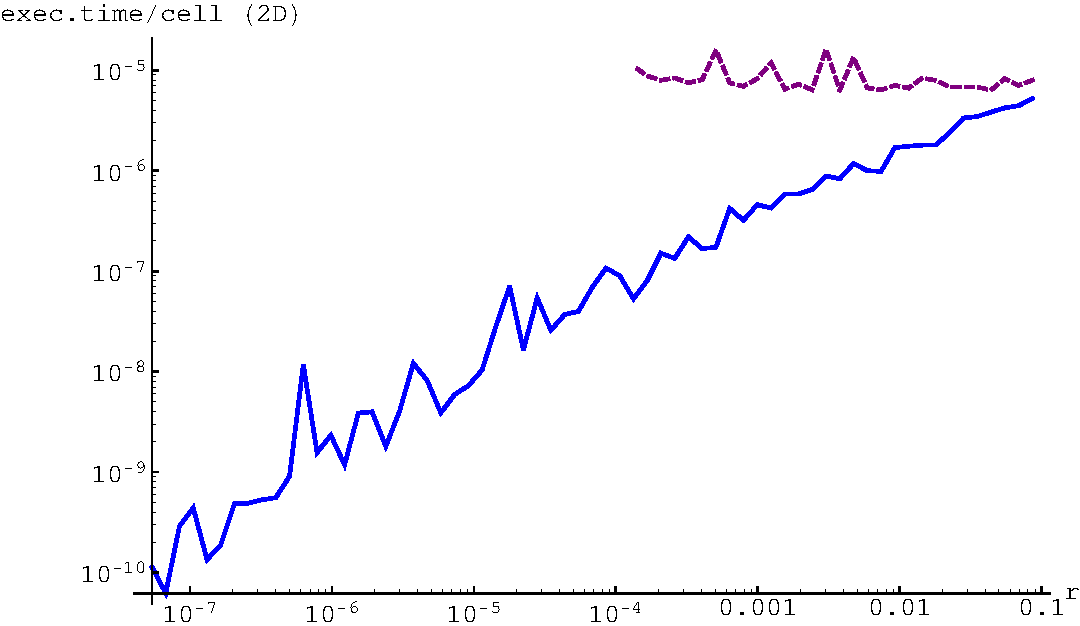
\includegraphics [width=260pt]{exectimepercell-2D.pdf}
\caption{Mean execution time per cell of finding the first collision in 2D Lorentz gas, for the classical (dashed curve) and efficient (solid curve) algorithms.}
\label{fig:exectimepercell2D}
\end{figure}

\begin{figure}
\centering
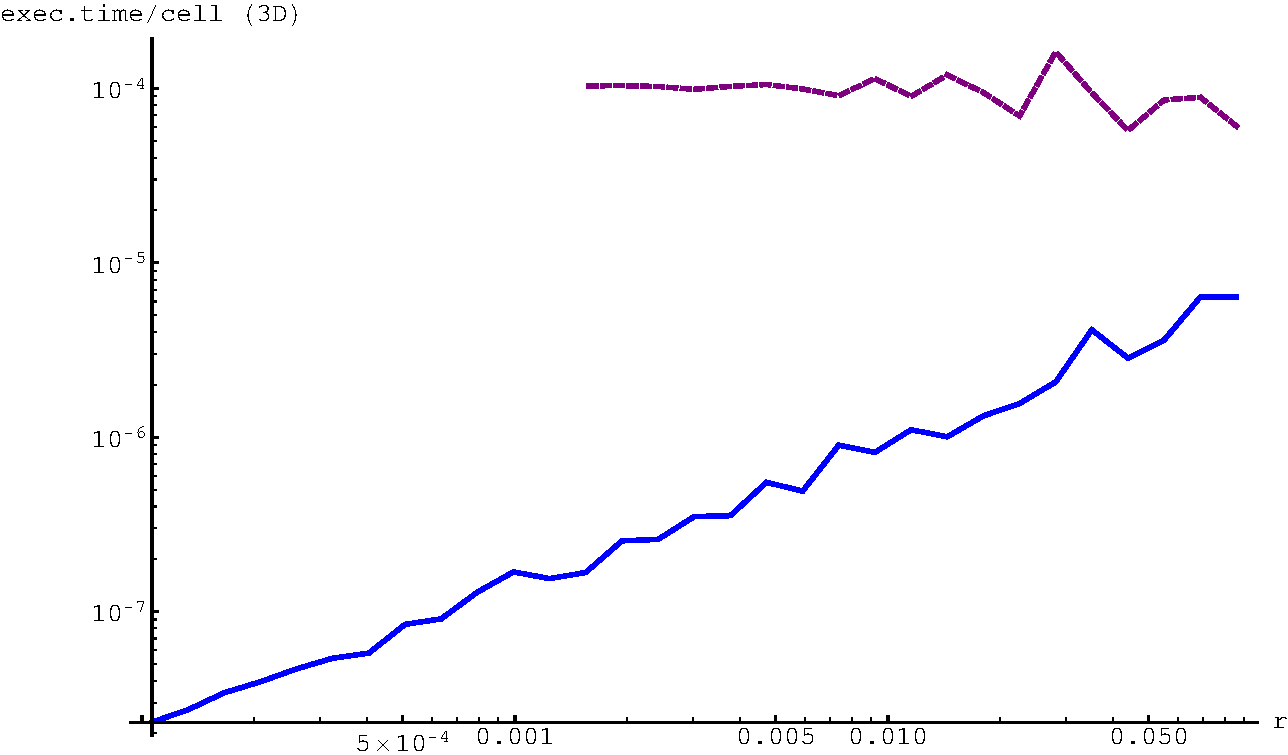
\includegraphics [width=260pt]{exectimepercell-3D.pdf}
\caption{Mean execution time per cell of finding the first collision in 3D Lorentz gas, for the classical (dashed curve) and efficient (solid curve) algorithms.}
\label{fig:exectimepercell3D}
\end{figure}

\subsection{Free flight distribution}
As an example application of our algorithm, we measure the distribution of free flight lengths for the first collision for certain systems studied by Marklof and Str\"ombergsson \cite{marklof2014power}. They proved that the asymptotic decay of the probability density for free flights for $N$ incommensurable, overlapping periodic Lorentz gases in the Boltzmann--Grad limit is $\sim \ell^{-N-2}$. It follows that the asymptotic density of the \emph{first} free flight should be 
$\rho(\ell) \sim \ell^{-N-1}$.

Figure~\ref{fig:free-flights} shows our numerical results for this distribution in the case of two and three overlapping lattices, compared to the asymptotic decay given by the rigorous result of \cite{marklof2014power}. 
To obtain this plot, we fixed the radius $r=10^{-4}$ and calculated free flights for a given initial condition for a 2D lattice, and for the same lattice rotated by $\pi/5$ and $\pi/7$, respectively. The first free flight for each lattice is calculated separately, and the minimum of those results is then taken to give the first free flight for the superposition of either two or three incommensurable lattices. 
The distributions obtained numerically do indeed follow the power laws predicted.  Naturally, it becomes increasingly difficult to obtain the asymptotic behaviour of the densities as the number of lattices increases.

\begin{figure}
\centering
\includegraphics*[width=280pt]{free_flight_distribution_incommensurable}%{Free-Fligth-Rot.pdf}
\caption{Probability density of the first free flight for two and three incommensurable, overlapping periodic Lorentz gases with angles $\pi/5$ and $\pi/7$; a total of $10^{8}$ initial conditions was used. The results for a single lattice are shown for comparison. The dashed lines and labels show the theoretical asymptotics.}
\label{fig:free-flights}
\end{figure}

\section{Conclusions}  

We have introduced efficient algorithms to simulate periodic Lorentz gases in two and three dimensions, that work particularly well when the obstacles are small. We have compared the efficiency of these algorithms with the standard ones, showing that the relative efficiency indeed increases very fast in 2D and fast in 3D, and we have shown a sample application to calculate free flight distributions in the Boltzmann--Grad limit.

The 3D algorithm can readily be generalized to higher dimensions; this is work in progress. 

\section{Acknowledgements}  
ASK received support within the Emmy Noether program (grant Schm
2657/2). NK is the recipient of a DGAPA-UNAM postdoctoral fellowship. DPS acknowledges financial support from CONACYT grant CB-101246 and DGAPA-UNAM PAPIIT grants IN116212 and IN117214. 

\appendix
\section{Approximation of an irrational number by a rational}

In this section we summarize some of the results on continued fractions used in the algorithm. The proofs can be found in books on number theory, e.g., 
\cite{niven2008introduction}. The geometrical interpretation has also been suggested before by many other authors; see, for example, \cite{nogueira1995three}. 

We define a continued fraction as follows:
A continued fraction is an expression obtained through an iterative process of representing a number $\alpha$ as the sum of its integer part $a_0$ and the reciprocal of another number $\alpha_1=\alpha-a_0$, then writing $\alpha_1$ as the sum of its integer part $a_1$ and the reciprocal of $\alpha_2=\alpha_1-a_1$, and so on:
\begin{equation*}
  \alpha = a_0 + \frac{1}{\displaystyle a_1
          + \frac{1}{\displaystyle a_2
          + \frac{1}{\displaystyle a_3 + \dots}}}
\end{equation*}

This expression produces a sequence of integers $\lfloor \alpha \rfloor=a_0$, $\lfloor \alpha_1 \rfloor=a_1$, $\lfloor \alpha_2 \rfloor=a_2$, etc. 
Then, we define inductively two sequences of integers $\{ p_n\}$ and $\{ q_n\}$ as follows:
%
\begin{eqnarray}
p_{-2} = 0;  \quad p_{-1} = 1;  \quad p_i &=a_i p_{i-1}+p_{i-2};
\label{eq:sucesion1}
\\ 
q_{-2} = 1,  \quad q_{-1} = 0,  \quad q_i &=a_i q_{i-1}+q_{i-2}.
\label{eq:sucesion2}
\end{eqnarray}

With this sequence we can approximate any irrational number $\alpha$ using the Hurwitz theorem:
For every irrational number $\alpha$ all the relative prime integers $p_n$, $q_n$ of the sequences defined in equations \eqref{eq:sucesion1} and \eqref{eq:sucesion2} satisfy 
\begin{equation}
|\alpha- \frac{p_n}{q_n}|\leq  \frac{1}{{q_n}^2}.
\end{equation}



%\bibliographystyle{apsrev}
\bibliographystyle{unsrt}
\bibliography{Bib-alg}


\end{document}
